\documentclass[12pt,letterpaper]{article}

\newenvironment{proof}{\noindent{\bf Proof:}}{\qed\bigskip}

\newtheorem{theorem}{Theorem}
\newtheorem{corollary}{Corollary}
\newtheorem{lemma}{Lemma} 
\newtheorem{claim}{Claim}
\newtheorem{fact}{Fact}
\newtheorem{definition}{Definition}
\newtheorem{assumption}{Assumption}
\newtheorem{observation}{Observation}
\newtheorem{example}{Example}
\newcommand{\qed}{\rule{7pt}{7pt}}

\newcommand{\assignment}[4]{
\thispagestyle{plain} 
\newpage
\setcounter{page}{1}
\noindent
\begin{center}
\framebox{ \vbox{ \hbox to 6.28in
{\bf CS412: ntroduction to Data Mining \hfill #1}
\vspace{4mm}
\hbox to 6.28in
{\hspace{2.5in}\large\mbox{Problem Set #2}}
\vspace{4mm}
\hbox to 6.28in
{{\it Handed Out: #3 \hfill Due: #4}}
}}
\end{center}
}

\newcommand{\solution}[4]{
\thispagestyle{plain} 
\newpage
\setcounter{page}{1}
\noindent
\begin{center}
\framebox{ \vbox{ \hbox to 6.28in
{\bf CS412:   Introduction to Data Mining \hfill #4}
\vspace{4mm}
\hbox to 6.28in
{\hspace{2.5in}\large\mbox{#3}}
\vspace{4mm}
\hbox to 6.28in
{#1 \hfill {\it #2}}
}}
\end{center}
\markright{#1}
}

\newenvironment{algorithm}
{\begin{center}
\begin{tabular}{|l|}
\hline
\begin{minipage}{1in}
\begin{tabbing}
\quad\=\qquad\=\qquad\=\qquad\=\qquad\=\qquad\=\qquad\=\kill}
{\end{tabbing}
\end{minipage} \\
\hline
\end{tabular}
\end{center}}

\def\Comment#1{\textsf{\textsl{$\langle\!\langle$#1\/$\rangle\!\rangle$}}}


%\documentclass{article}
\usepackage{amsmath}
\setlength{\parindent}{0pt}
\usepackage{graphicx}
\usepackage{ctable}
%\usepackage{fullpage}
%\usepackage{setspace} 
\usepackage{float}
%\usepackage{listings} 
%\usepackage{bbm}
\usepackage{bigstrut}
%\usepackage{caption}
%\usepackage{subcaption}
%\usepackage{algpseudocode}
%\usepackage{algorithm}

\usepackage{listings}
\usepackage{color}
\usepackage[utf8]{inputenc}

\definecolor{dkgreen}{rgb}{0,0.6,0}
\definecolor{gray}{rgb}{0.5,0.5,0.5}
\definecolor{mauve}{rgb}{0.58,0,0.82}

\lstset{frame=tb,
  language=matlab,
  aboveskip=3mm,
  belowskip=3mm,
  showstringspaces=false,
  columns=flexible,
  basicstyle={\small\ttfamily},
  numbers=none,
  numberstyle=\tiny\color{gray},
  keywordstyle=\color{blue},
  commentstyle=\color{dkgreen},
  stringstyle=\color{mauve},
  breaklines=true,
  breakatwhitespace=true,
  tabsize=3
}


\oddsidemargin 0in
\evensidemargin 0in
\textwidth 6.5in
\topmargin -0.5in
\textheight 9.0in
\usepackage{multirow}
\usepackage{hyperref}

\hypersetup{colorlinks=true}
\usepackage{color}

%\newcommand{\ans}[1]{{[{\sc Answer:} {\sf #1}]}}
\newcommand{\ans}[1]{}

\begin{document}


\solution{Li Miao}{\today}{Assignment 3}{Fall 2015}
% Fill in the above, for example, as follows:
% \solution{Joe Smith}{\today}{1}{Fall 2012}

\pagestyle{myheadings}  % Leave this command alone

\paragraph*{General Instruction}
\begin{itemize}
\setlength{\itemsep}{2pt}
\item Errata: After the assignment is released, any further corrections of errors or clarifications will be posted at \href{https://piazza.com/class/idqujg4tiae3q0?cid=152}{the Errata page at Piazza}. Please watch it.
\item Feel free to talk to other members of the class when doing the homework. We are more concerned about
whether you learn how to solve the problem than whether you solve it entirely on your
own. You should, however, write down the solution yourself. 
\item Please use Piazza first if you have questions about the homework. Also feel free to send us e-mails and come to office hours. 
\item For each question, you will \textbf{NOT} get full credit if you only give a final result. Necessary calculation steps and reasoning are required. 
\item For each question, you should show the necessary calculation steps and reasoning---not only final results. Keep the solution brief and clear.
\item For a good balance of cognitive activities, we label each question with an activity type:
\begin{itemize}
\item {\bf L1 (Knowledge)} Definitions, propositions, basic concepts.
\item {\bf L2 (Practice)} Repeating and practicing algorithms/procedures.
\item {\bf L3 (Application)} Critical thinking to apply, analyze, and assess.
\end{itemize}
\end{itemize}

\paragraph*{Assignment Submission}
\begin{itemize}
\setlength{\itemsep}{2pt}
\item Please submit your work before the due time. \textbf{We do NOT accept late homework!}
\item Please submit your answers electronically via Compass (\url{http://compass2g.illinois.edu}). Contact TAs if you have technical difficulties in submitting the assignment.
\item Please {\bf type} your answers in an \textbf{Answer Document}, and submit it in PDF. \textbf{Handwritten answers or hand-drawn pictures} \textbf{are not acceptable}. 
\item This assignment consists of four written assignments and one large Machine Problem (MP). Your answers to all questions (including MP) should be included in one Answer Document, named as {\tt NetId\_assign3\_answer.pdf}.
\item The four written questions do not require programming at all. The last part is the first MP (not a mini one) we have in this course. It consists of several programming assignments, which usually take more time than written assignments, so please \textcolor{red}{start early}.
\item Find detailed submission guidelines for codes and results in the requirements of MP.

\end{itemize}

\section*{Question 1 (12 points)}
Based on the tiny database of 5 transactions in Table 1, use the Apriori algorithm to find the frequent patterns with \textcolor{red}{relative $min\_sup=0.6$}.\\

\textbf{Purpose} 
\begin{itemize}
\item Get a better understanding as well as hands-on experience of the Apriori algorithm.
\end{itemize}

\textbf{Requirements}
\begin{itemize}
\item For this question, you are required to simulate the basic Apriori algorithm and write down all intermediate as well as final results. No programming is needed. 
\item Use the abbreviations we give you (C1, F1...) to denote which list you are writing about. You may use a table to contain all lists, or just write them one by one.
\item For each itemset you write down in the F$i$ lists, put its corresponding absolute support after it, with a colon between them, such as $F1 = \{ m:4, \ldots\}$.
\item Do not forget to write down the actions (pruning or self-joining) you take to generate F1 and C2.
\end{itemize}

\begin{table}[h!]
\begin{center}
\begin{tabular}{lr}
\toprule
Trans. &Items  \\ \hline 
$1$ &b,d,f,g,l  \\ 
$2$ &f,g,h,l,m,n  \\
$3$ &b,f,h,k,m  \\ 
$4$ &a,f,h,j,m  \\ 
$5$ &d,f,g,j,m  \\ 
\bottomrule
\end{tabular}
\caption{A tiny transaction database}
\end{center}
\end{table}

\begin{itemize}
\item[a.] $(2', L1)$ We do db-scanning to get rid of non-frequent 1-itemsets

\begin{figure}[H]
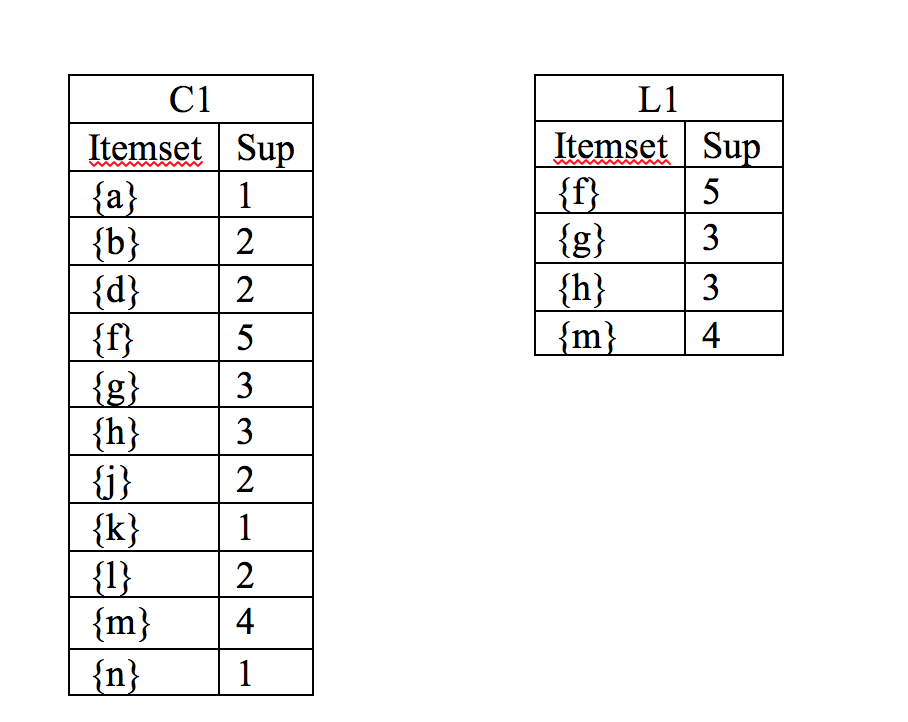
\includegraphics[width=0.5\textwidth]{Figures/C1.png}
\centering
\end{figure}

\item[b.] $(2', L1)$ We do self-joining to generate all candidate 2-itemsets

\begin{figure}[H]
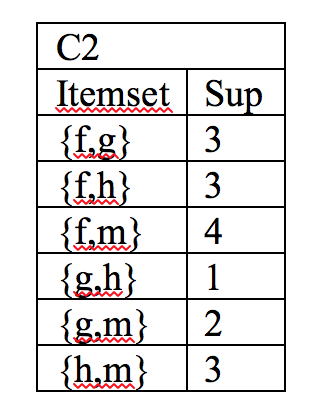
\includegraphics[width=0.2\textwidth]{Figures/C2.png}
\centering
\end{figure}

\item[c.] $(2', L1)$ 

\begin{figure}[H]
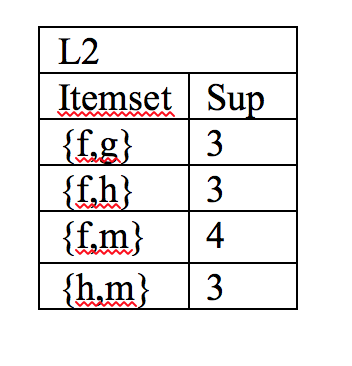
\includegraphics[width=0.2\textwidth]{Figures/L2.png}
\centering
\end{figure}

\item[d.] $(2', L1)$ We need pruning. 

\begin{figure}[H]
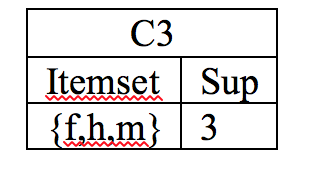
\includegraphics[width=0.2\textwidth]{Figures/C3.png}
\centering
\end{figure}


\item[e.] $(2', L2)$ There is no frequent 4-itemset. Because we only have one frequent 3-itemset.

\item[f.] $(2', L3)$  I think the self-joining involves the heaviest computation. We need to generate so many joint candidates. When $min\_sup$ is really low, we need to consider more itemsets. Therefore it would be extremely bad. $M^N$ where M is number of distinct items and N is the max length of transactions
\end{itemize}


\section*{Question 2 (13 points)}
Based on the same database Question 1, use the Frequent Pattern Growth algorithm with \textcolor{red}{relative $min\_sup=0.4$} to find the frequent patterns.\\

\textbf{Purpose}
\begin{itemize}
\item Get a better understanding as well as hands-on experience of the FP-Growth algorithm.
\end{itemize}

\textbf{Requirement}
\begin{itemize}
\item For this question, you are required to simulate the basic FP-Growth algorithm. No programming is needed.
\item You are required to generate some tables and figures. You can use any software to do that, but you can not draw with hand and then scan or take photos. 
\item For sub-question a, generate a table to present the results.
\item For sub-question b, put the Header Table and FP-tree side by side, preferably with Header Table on the left (just like those in the slides). Use a colon to separate an item and its corresponding count in the FP-tree.
\item For sub-question c, for each of the items, write down its Conditional Pattern Base followed by the frequent patterns computed based on it. In order to generate the correct frequent patterns, please first generate the Conditional FP-trees. But you do not need to show the Conditional FP-trees in the Answer Document.
\end{itemize}

\begin{enumerate}
  \item[a.] $(2', L2)$ 
  \begin{figure}[H]
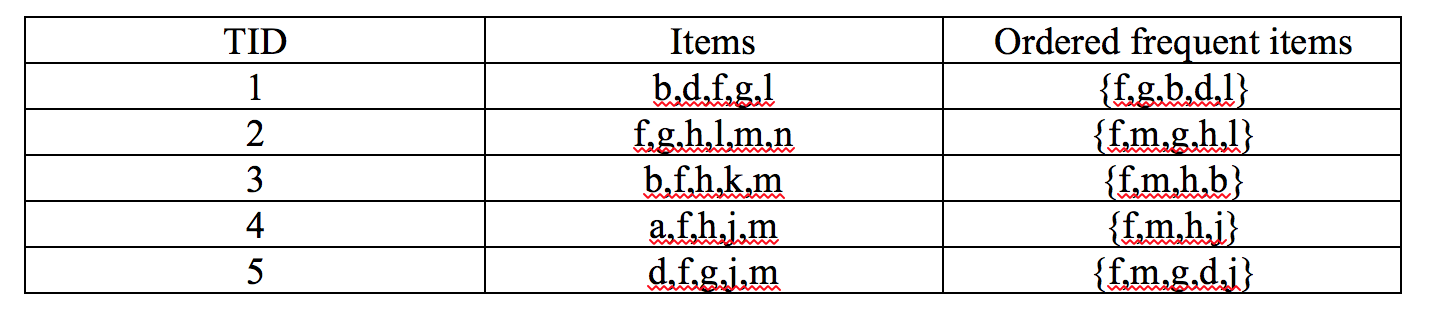
\includegraphics[width=0.8\textwidth]{Figures/order.png}
\centering
\end{figure}


  \item[b.] $(5', L2)$ 
  \begin{figure}[H]
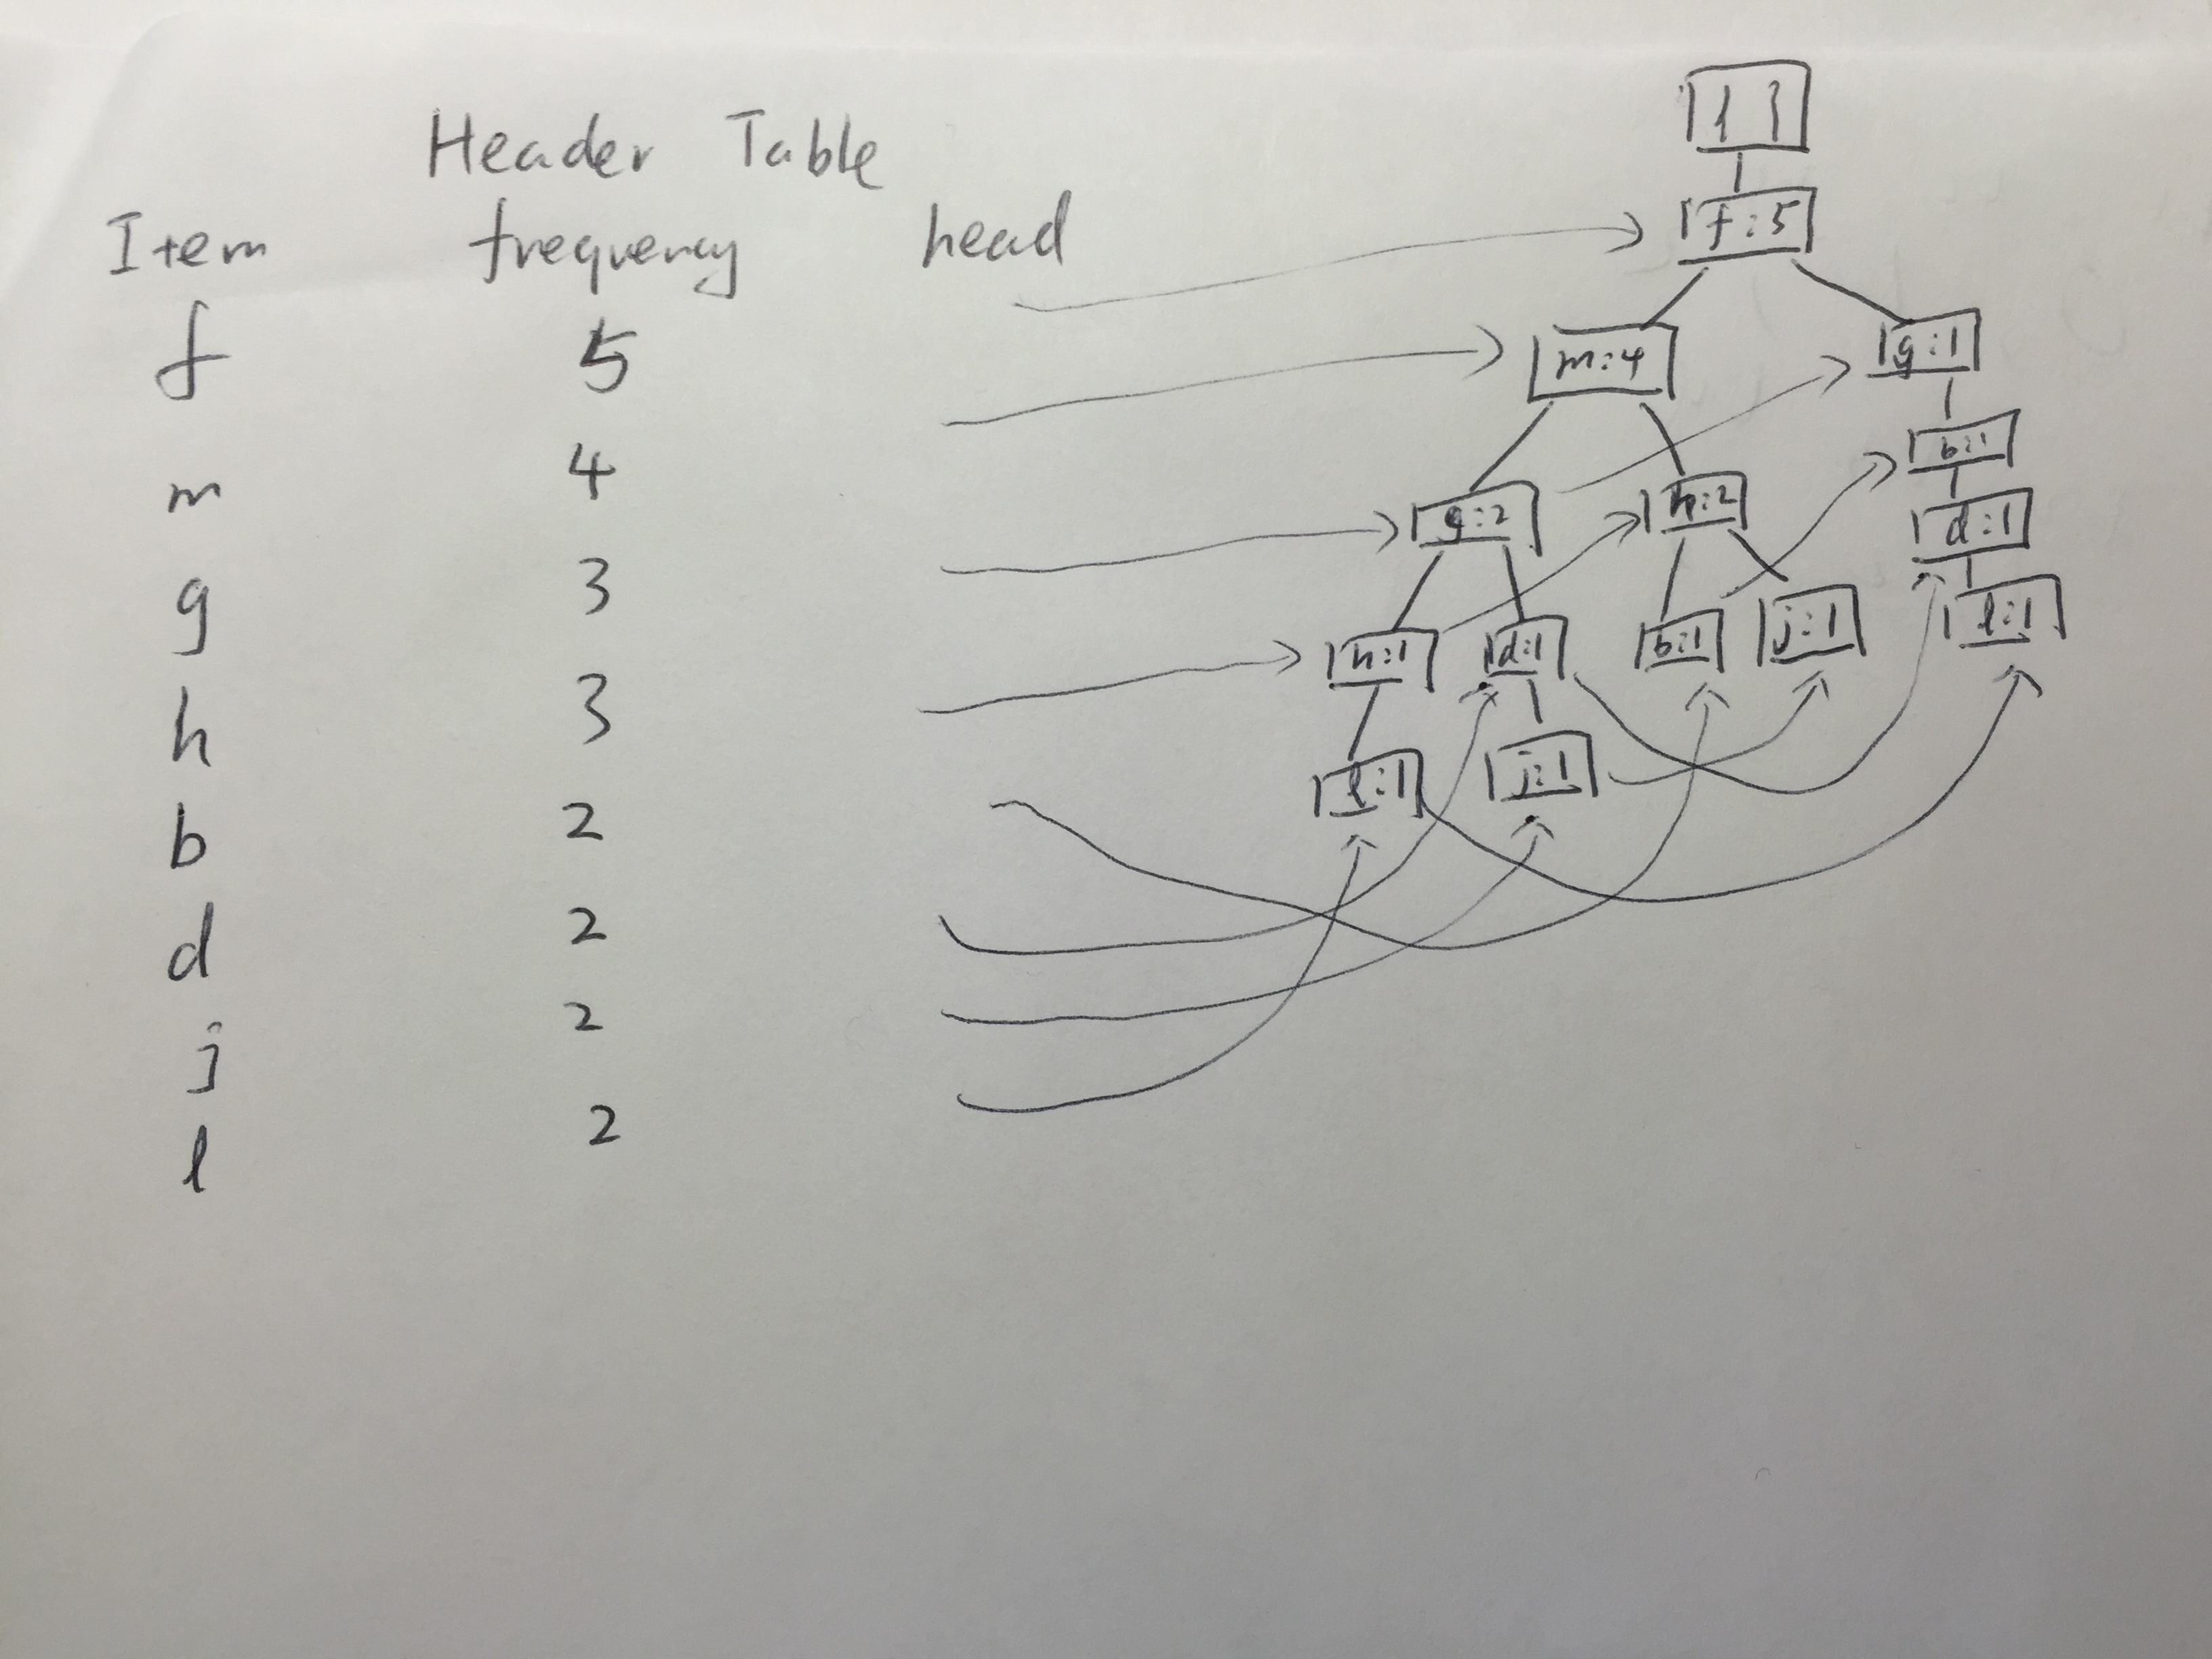
\includegraphics[width=0.8\textwidth]{Figures/header.png}
\centering
\end{figure}

  \item[c.] $(4', L2)$ 
  
    \begin{figure}[H]
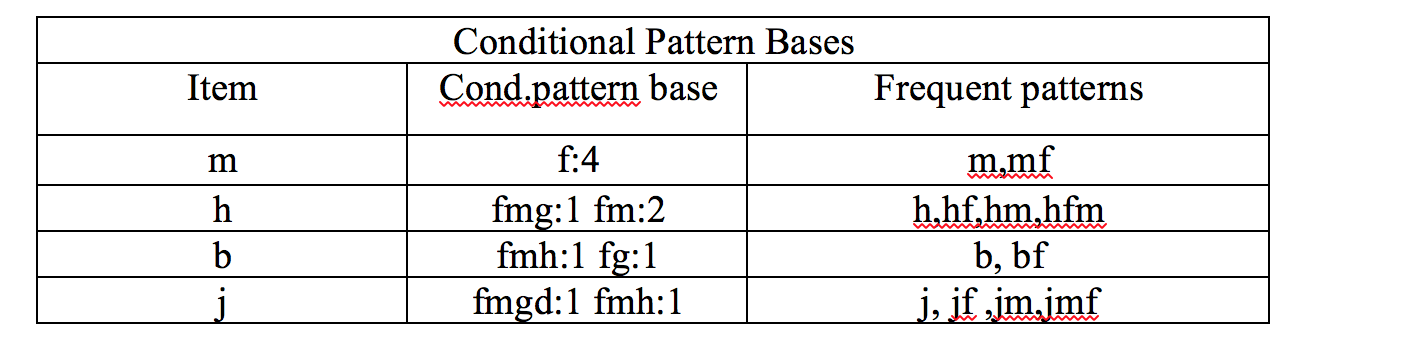
\includegraphics[width=0.8\textwidth]{Figures/cond.png}
\centering
\end{figure}
  
  \item[d.] $(2', L3)$ We hope to use FP tree to compress our database. When we order items according to the frequency, we can make the tree smaller. So it will be more efficient and save the computation cost.
  
\end{enumerate}


\section*{Question 3 (10 points)}
Based on the frequent patterns computed in Question 1, find closed patterns, maximal patterns and association rules. \\ 

\textbf{Purpose}
\begin{itemize}
\item Get a better understanding of closed patterns, maximal patterns and association rules.
\end{itemize}

\textbf{Requirement}
\begin{itemize}
\item For this question, you will be doing some counting. No programming is needed.
\item For sub-question c, show the relative support and confidence of each association rule you find.
\end{itemize}

\begin{enumerate}
  \item[a.] $(3', L1)$ Closed: f, fg ,fm, fhm
  
  \item[b.] $(3', L1)$ Maximal: fg, fhm

  \item[c.] $(2', L2)$ 
  
  \begin{itemize}
  \item $g \to f$ (0.6,1)
  \item $h \to f$ (0.6,1)
  
  \end{itemize}
  
  \item[d.] $(2', L3)$ Max implies closed, but not versa vice. So if we only hope to get the general idea of frequent patterns, like what items would like to show up together, we may choose Max. But if we hope to get more details, we would choose closed patterns. 
  
  
\end{enumerate}


\section*{Question 4 (15 points)}
This is a set of \textbf{true} or \textbf{false} questions.  Please answer the following questions. \\ 

\textbf{Purpose}
\begin{itemize}
\item Have a better understanding of some basic concepts about frequent pattern mining.
\end{itemize}

\textbf{Requirement}
\begin{itemize}
\item For each sub-question, choose \textbf{true (T)} or \textbf{false (F)} and provide a brief explanation of your choice. You will not get credit without explanation. 
\end{itemize}

\begin{enumerate}
  \item[a.] $(3', L3)$ T. Max means support(super(x)) $<$ $mim\_support$ $<= $support(x) ,and Closed means support(super(x)) $< $support(x). It is obvious that max implies closed, but not versa vice. 
  \item[b.] $(3', L2)$ F. When K =1, this statement is not true. Because(K-1) = 0. And to remove infrequent items, we also use pruning, not just scanning the database.
   \item[c.] $(3', L2)$ F. For FP-Growth, in order to mine all frequent patterns, we have to recursively generate conditional frequent bases and conditional FP-trees until the FP-tree generated has single path.
 \item[d.] $(3', L1)$ F. CLOSET is based on FP-Growth while MaxMiner is based on Apriori.
 \item[e.] $(3', L3)$ F. Support and confidence are not good to indicate correlations. But we cannot say Lift is always better. We can see the obvious example on textbook. The Lift is low but there is a clear association relationship for D2.  We can use support and confidence to find interesting association rules. 
     \begin{figure}[H]
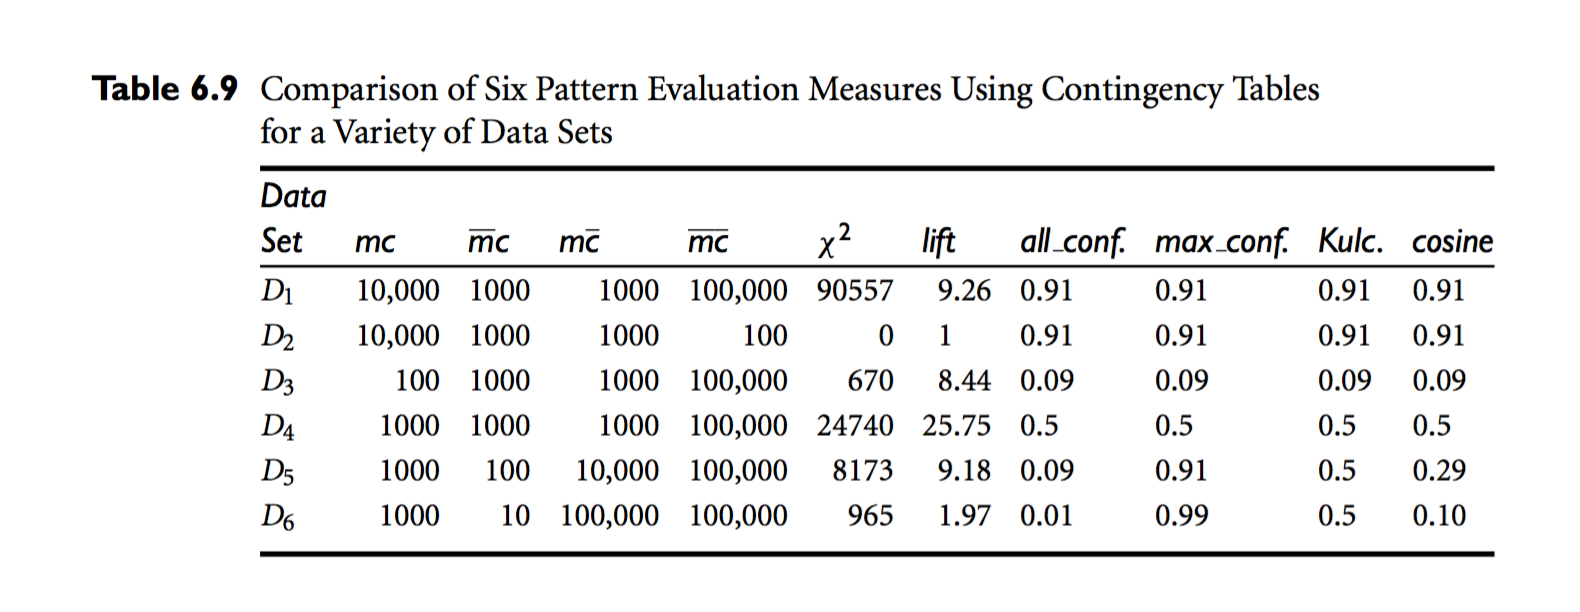
\includegraphics[width=0.8\textwidth]{Figures/lift.png}
\centering
\end{figure}
 
\end{enumerate}


\section*{Machine Problem (MP, 50 points)}
Computing frequent patterns by hand is so tedious - this is where computers come into use! 

In this MP, given preprocessed data of the paper titles collected from computer science conferences from 5 domains, you are required to 1) implement a frequent pattern mining algorithm to mine frequent patterns from each of the 5 domains, so as to find `meaningful' patterns for each domain;  2) mine closed/maximal patterns based on the frequent patterns you find, so as to understand the different definitions and applications of closed/maximal patterns; 3) find association rules using Weka. You can find {\tt data.zip} from \href{https://wiki.cites.illinois.edu/wiki/display/cs412fa15/Assignments}{the course website}.\\ 

\textbf{Description of Data Preprocessing}
\begin{itemize}
\item We use paper titles collected from conferences in computer science of 5 domains: Data Mining (DM), Machine Learning (ML), Database (DB), Information Retrieval (IR) and Theory (TH). The raw data is named as \textcolor{red}{\tt paper\_raw.txt}. Each line contains two columns, the {\tt PaperID} and the {\tt Title} of a paper, separated by a tab. Recall the example in class. You can consider each line in the file as one transaction. Each term in the title is then equivalent to an item in a transaction. We provide this file to give you a basic idea about what the task is and what data you are using. \textcolor{red}{You will not work on this file directly.}
\item For this assignment, we have pre-processed the raw data by removing stop words, converting the words to lower cases, and lemmatization. The results are in \textcolor{red}{\tt paper.txt}. In this file, each line is a list of terms. Terms are separated by one space. Again, this file is for you to understand the task, and \textcolor{red}{you will not work on this file directly.}
\item To make computation easier, we generate a vocabulary from {\tt paper.txt}, and name it as \textcolor{red}{\tt vocab.txt}. Each line in this file has two columns: the first column is the term index and the second column is a unique term extracted from {\tt paper.txt}; columns are separated by Tab. Each term in {\tt paper.txt} appears exactly once in {\tt vocab.txt}. With this vocabulary, we can always map between each term and its corresponding unique indexing number. \textcolor{red}{You do not need to know how this vocabulary is generated, but you do need this file to show mined patterns as required in Step 1 and Step 2 of the MP.}
\item Recall we have papers from 5 domains. We want you to mine frequent patterns for each of the 5 domains so as to find `meaningful' patterns of each domain. However, the terms of 5 domains are mixed together in {\tt paper\_raw.txt} and {\tt paper.txt}. In order to separate them, we apply \href{https://en.wikipedia.org/wiki/Latent_Dirichlet_allocation}{LDA} with 5 topics to assign one topic to each term. Then we re-organize the terms and create one file {\tt topic-$i$.txt} for each topic $i$, where $i=0,1,2,3,4$. Each line in file {\tt topic-$i$.txt} corresponds to one paper title in the dataset. File {\tt topic-$i$.txt} only contains paper titles with at least one term assigned with topic $i$ by LDA, and within each paper title in {\tt topic-$i$.txt}, terms assigned with topics other than topic $i$ are removed. Note that we do not know which {\tt topic-$i$.txt} corresponds to which of the 5 domains now, and we will use frequent pattern mining to figure it out. \textcolor{red}{These {\tt topic-$i$.txt} are the files you are going to work on to mine frequent patterns.}
\end{itemize}

\begin{enumerate}
\item[Step 1:] $(25', L3)$ \textbf{Mining frequent patterns for each topic.} 
  
Question to ponder A: How do you choose min\_sup for this task? Explain your criteria; any reasonable choice will be good.

Answers: I choose the {\it min\_sup} to be $1\%$ of the dataset. It is a reasonable assumption because we will not have too many items to combine or miss some interesting frequent patterns when we set the {\it min\_sup} to be $1\%$ of the dataset.
  
\item[Step 2:] $(20', L3)$ \textbf{Mining closed/maximal patterns.} 

Question to ponder B: Can you figure out which topic corresponds to which domain based on patterns you mine? Write down your observations.

Answers: The topic-0 file corresponds to Data Mining. The topic-1 file corresponds to Machine Learning. The topic-2 file corresponds to Information Retrieval . The topic-3 file corresponds to Database. The topic-4 file corresponds toTheory. 

Question to ponder C: Compare the results of frequent patterns, closed patterns and maximal patterns, is there any difference? If so, what kind of patterns give more satisfying results? Write down your analysis.

Answers: Yes. There are some difference among the results from frequent patterns, closed patterns and maximal patterns. The results from closed patterns and frequent patterns are similar. For maximal patterns, the result files include fewer items than closed patterns or frequent patterns. I think the the frequent patterns give more satisfying results because it capture most key words for the specific domain and exclude some redundant information. And we can easily to figure which topic corresponds to which domain by frequent patterns.
 
\item[Step 3:] $(5', L2)$  \textbf{Mining association rules by Weka.} 

In this step, you will use Weka to mine association rules. In class, we have demonstrated how to do this. You can download the slides \textit{Weka-Associate} from the course schedule page or watch the online lecture video to review the process. To make things easier, we also provide detailed procedures here. 
%Pictures

   \begin{figure}[H]
   \caption{For topic-0,$min\_sup = 0.01$, $min\_conf = 0.3 $}
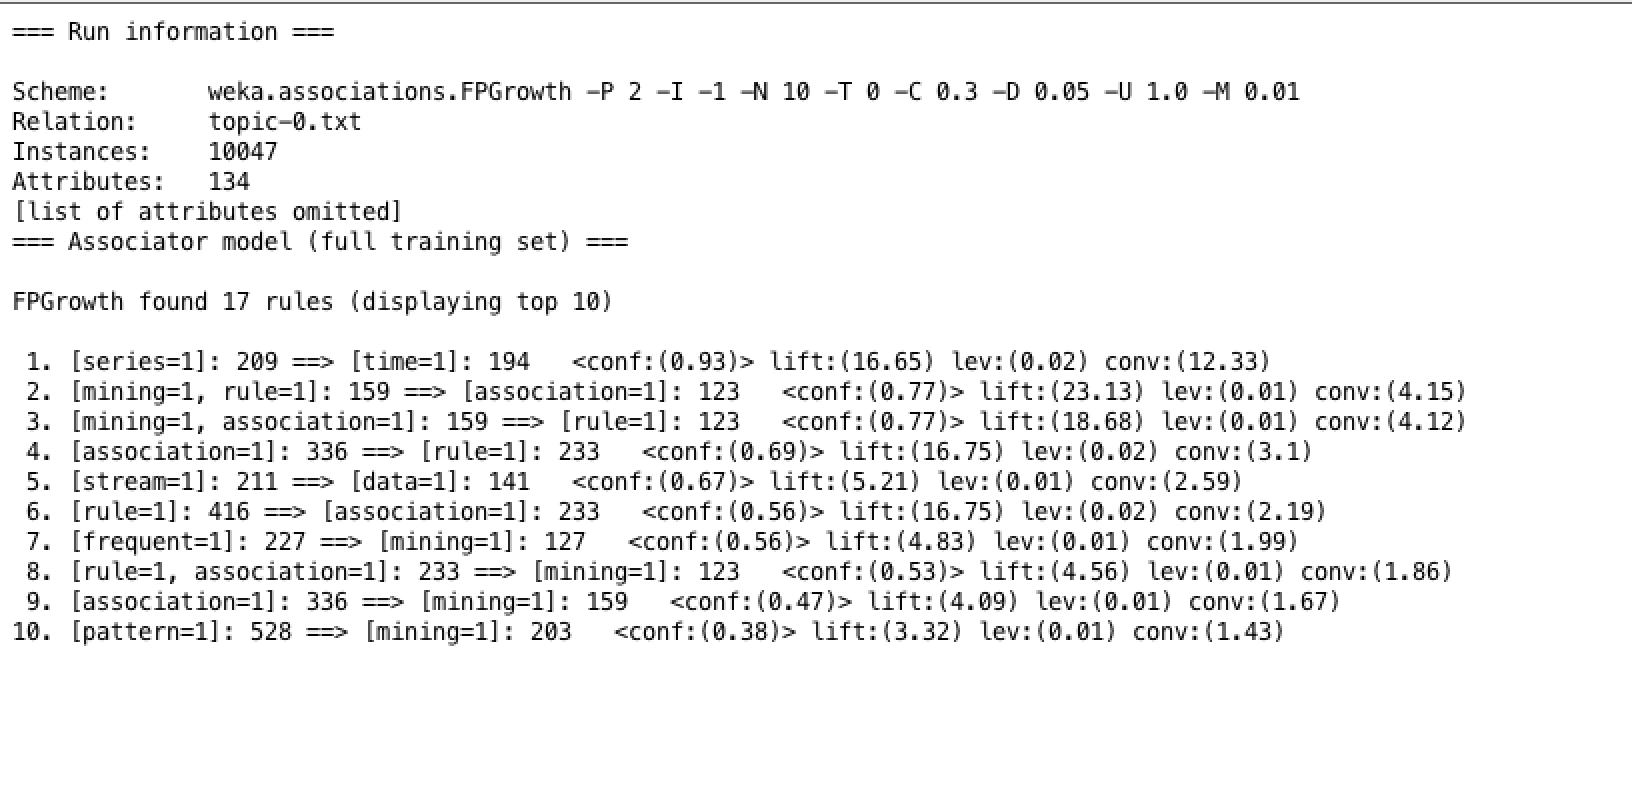
\includegraphics[width=0.8\textwidth]{Figures/0.png}
\centering
\end{figure}

   \begin{figure}[H]
     \caption{For topic-1,$min\_sup = 0.01$, $min\_conf = 0.5 $}
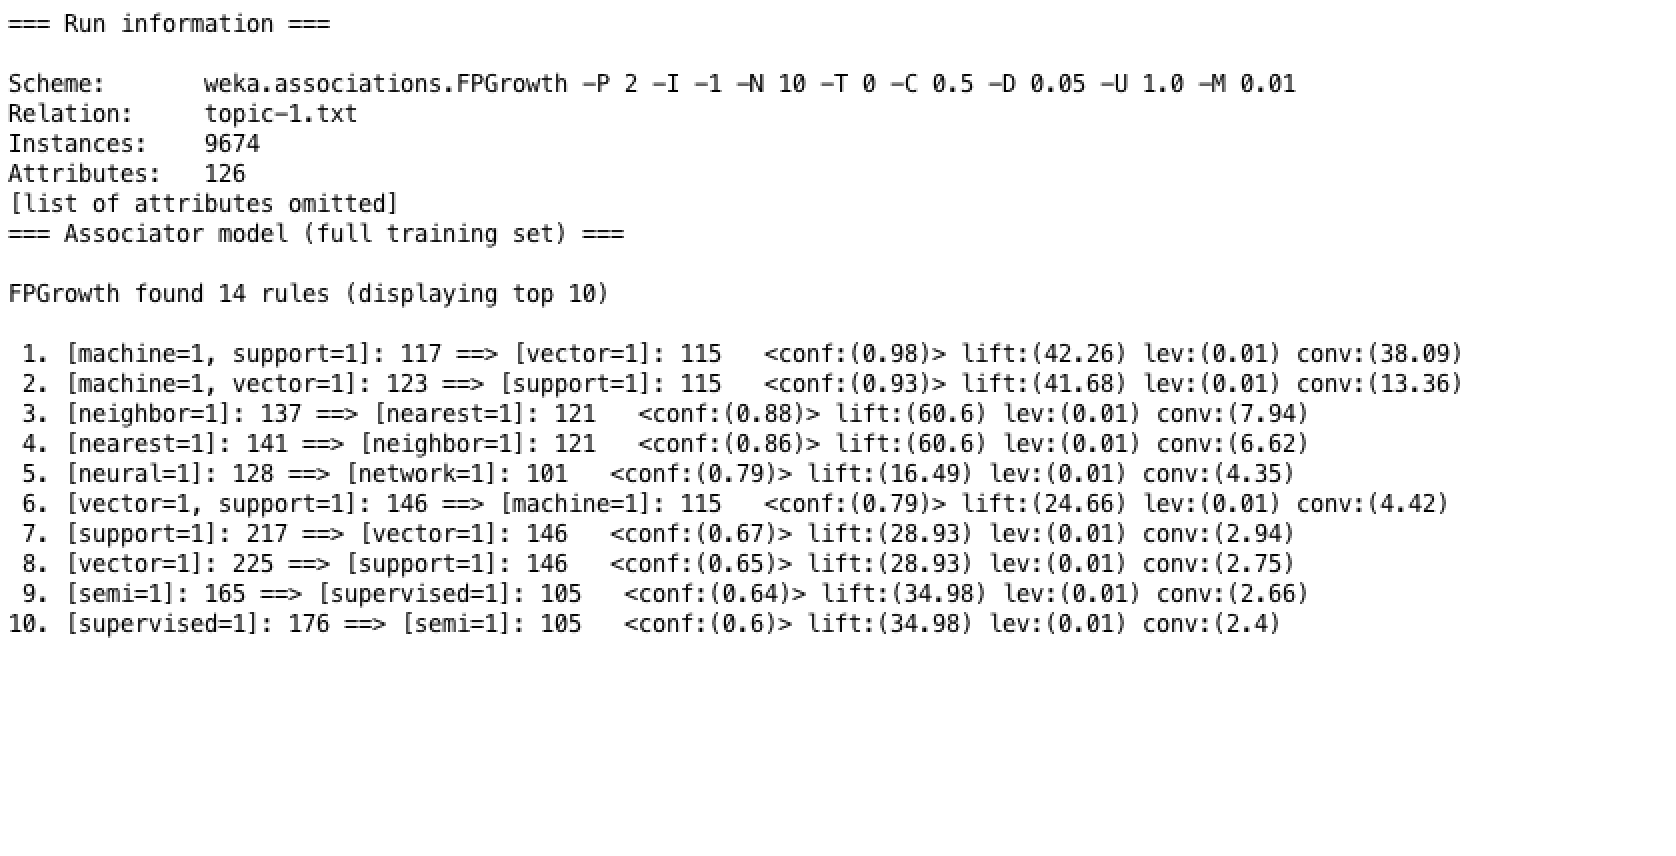
\includegraphics[width=0.8\textwidth]{Figures/1.png}
\centering
\end{figure}

   \begin{figure}[H]
     \caption{For topic-2,$min\_sup = 0.01$, $min\_conf = 0.2 $}
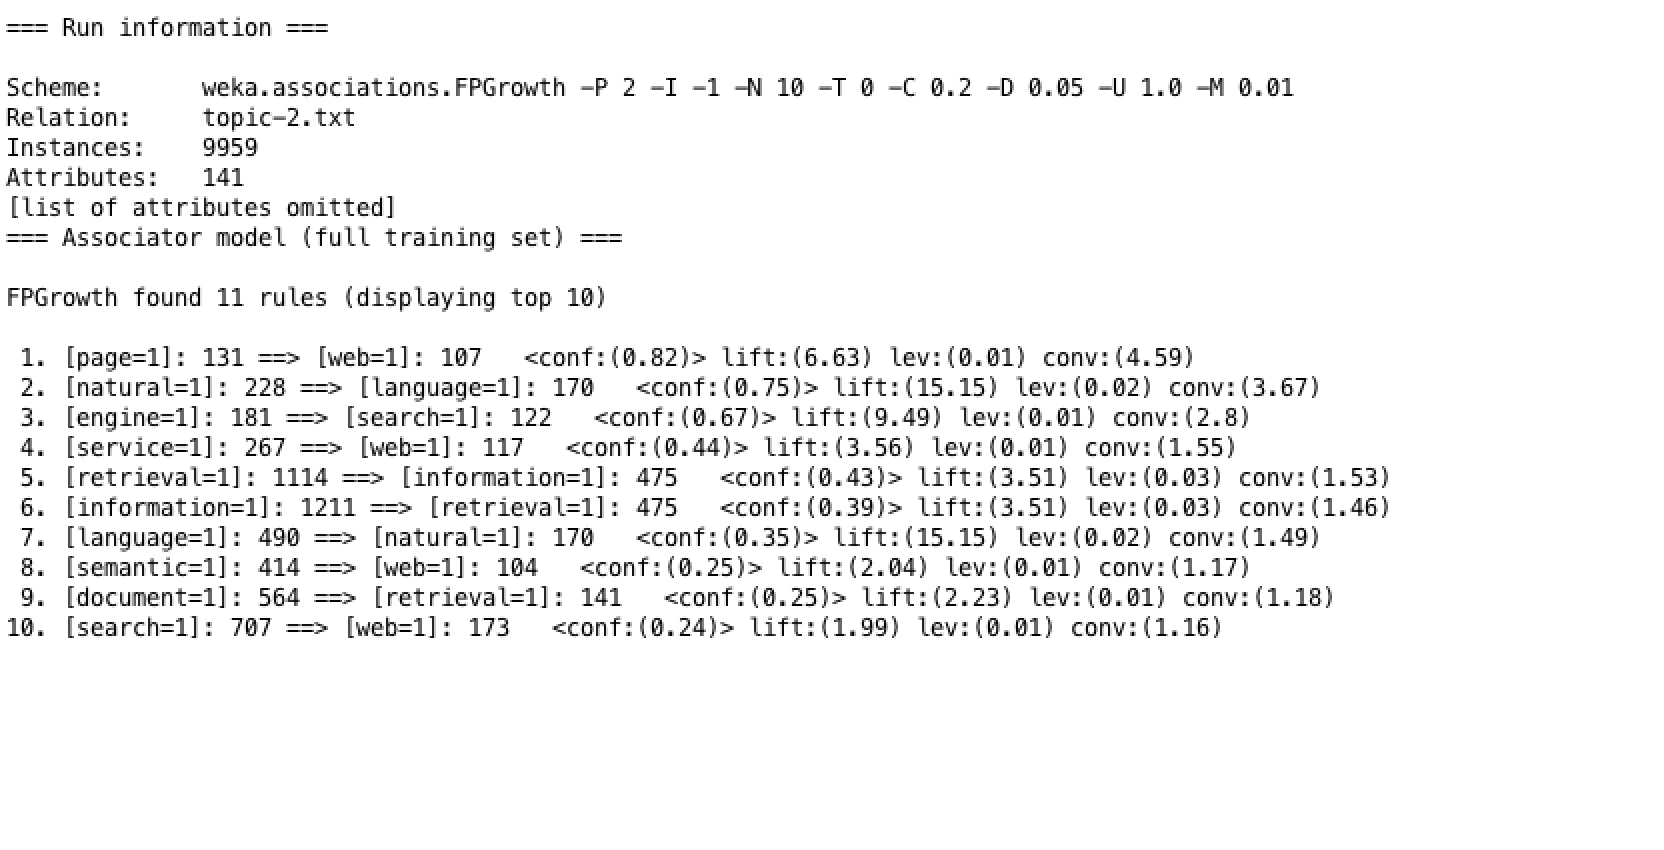
\includegraphics[width=0.8\textwidth]{Figures/2.png}
\centering
\end{figure}

   \begin{figure}[H]
     \caption{For topic-3,$min\_sup = 0.01$, $min\_conf = 0.2 $}
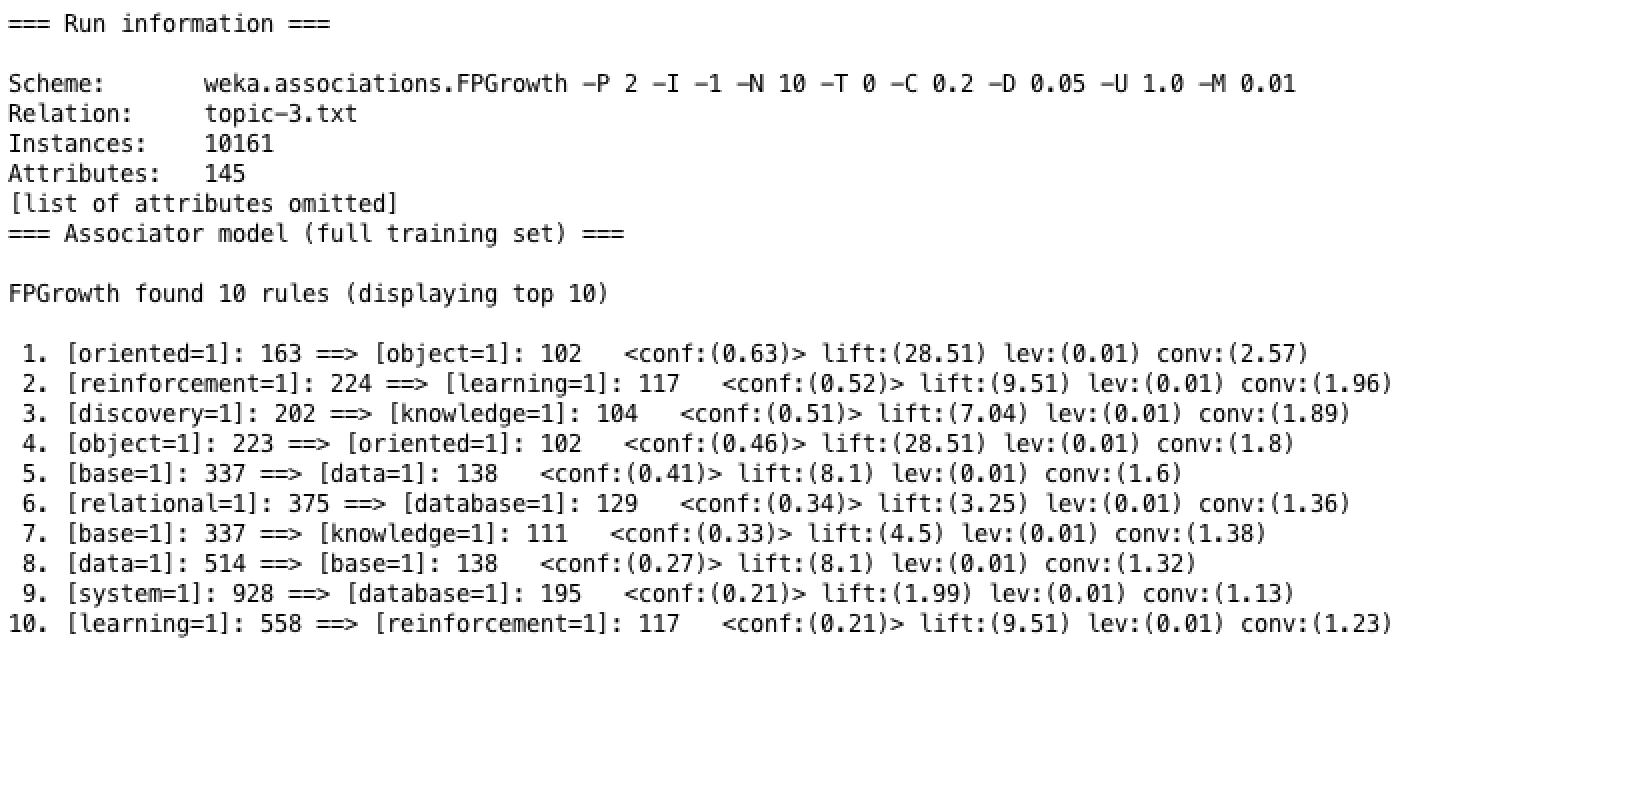
\includegraphics[width=0.8\textwidth]{Figures/3.png}
\centering
\end{figure}

   \begin{figure}[H]
     \caption{For topic-4,$min\_sup = 0.01$, $min\_conf = 0.28 $}
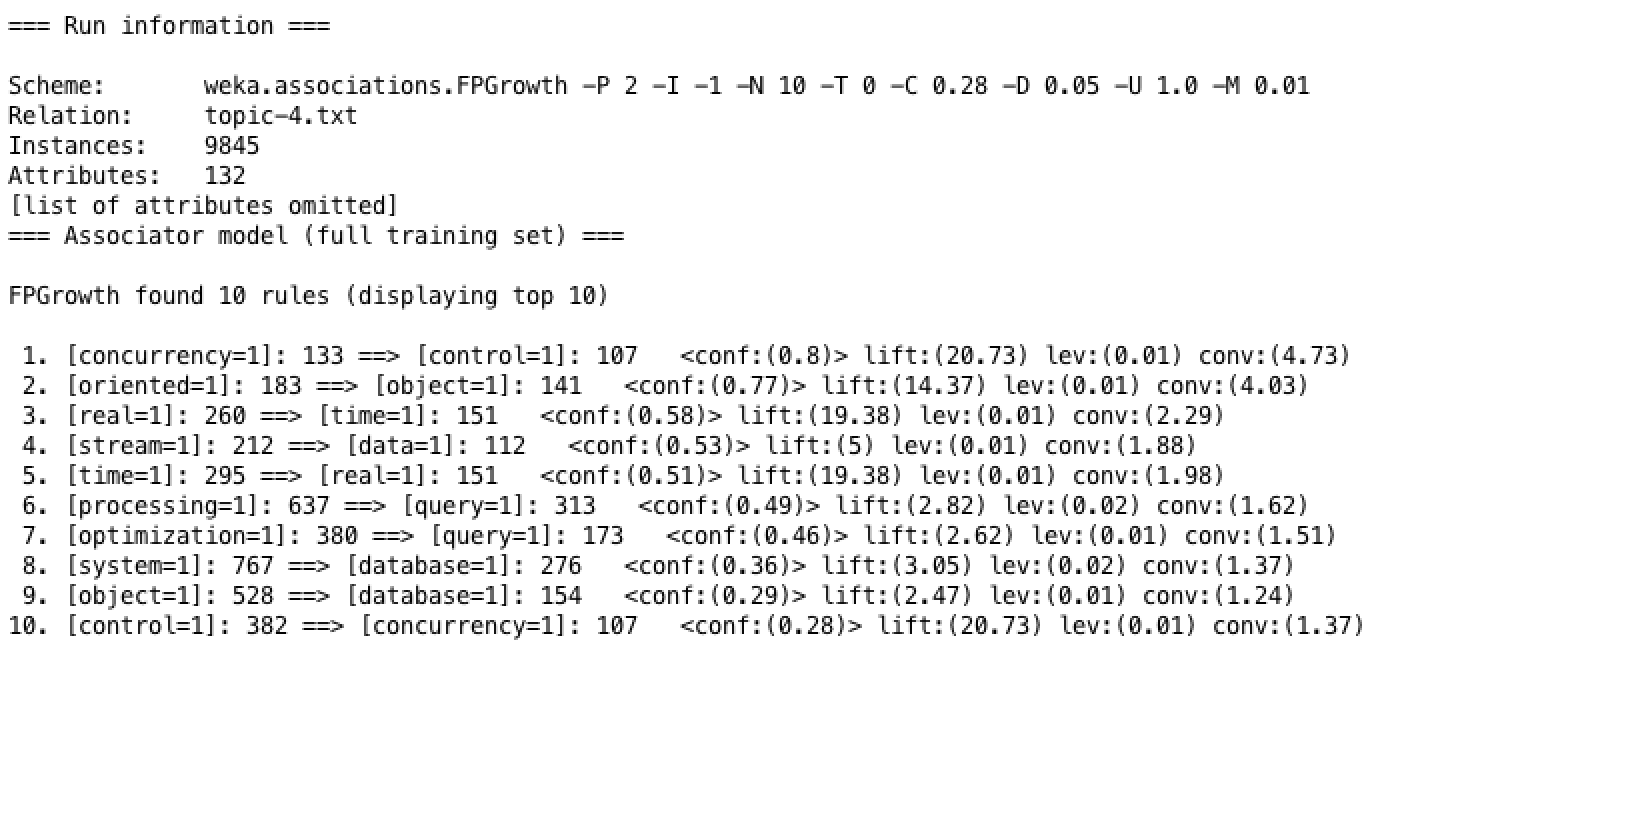
\includegraphics[width=0.8\textwidth]{Figures/4.png}
\centering
\end{figure}

Question to ponder D: What are the differences between phrases which satisfy only the {\it min\_sup} criterion and phrases (association rules) which satisfy both {\it min\_sup} and {\it min\_conf} criteria? Compare the results of Step 1 and Step 3 and write down your observations.

Answers: If we hope the phrases to satisfy both {\it min\_sup} and {\it min\_conf}, we hope to find some association rules and it is the stricter requirement. But when we only need the {\it min\_sup} to be satisfied, we just hope to find some interesting frequent patterns. And we do not know exactly the association or the causality between items. 

\end{enumerate}

\end{document}